\documentclass[10pt]{article}
\usepackage{graphicx}
\usepackage{float}
\usepackage{subfig}
\usepackage{color}
\usepackage{epsf,amsmath,amssymb,amsfonts}


\include{Wendy_macros}
\title{Result figures}
\begin{document}

\maketitle


In this paper, I will do every test based on combinations of two different line search seperately.
\begin{itemize}
\item 1st approach of line search: choose $\alpha_{0}$ as the minimum of feasible steps based on every variable, denoted as $lin1$
\item 2nd approach of line search: Fix $\alpha_{0}=1$, then apply Armijo, denoted as $lin2$
\item 3rd approach of line search:  Fix $\alpha_{0}=1$, then apply Armijo. Also fix the binding points without moving, denoted as $lin3$.
\end{itemize}

\section{TN: lin1; MG/OPT: lin3}

In Fig \ref{fig:coarse}, figure \ref{fig:vsc} illurstrates how close among the exact original prolem solution (green), solution of shifted problem  (red), approximation from fine solution (blue); 
figure \ref{fig:direction} is showing the error with these three solution. 

\begin{figure}
  \centering
  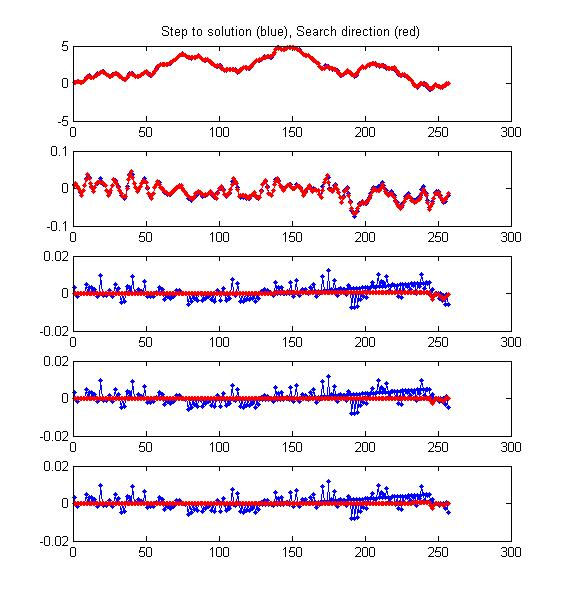
\includegraphics[width=1\textwidth]{finedirvs13}
  \caption{2-side bounds: TN: lin1; MG/OPT: lin3; Compare step to solution with search direction on fine level: discretization level: $[257,128]$}
  \label{fig:fine13}
\end{figure}


\begin{figure}
  \centering
  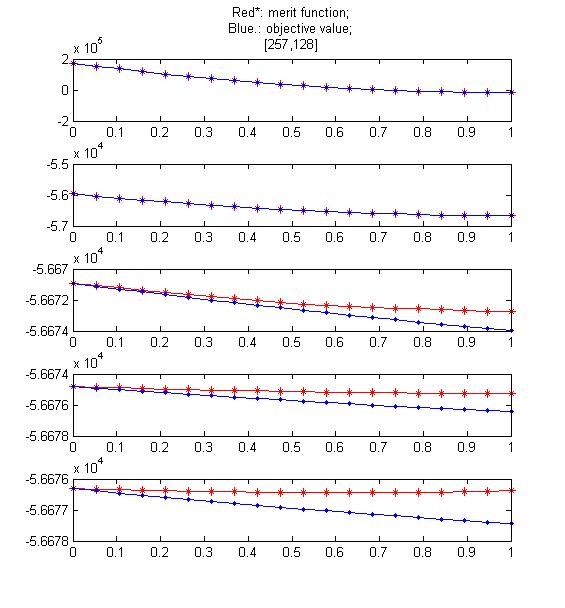
\includegraphics[width=1\textwidth]{merit13}
  \caption{2-side bounds: TN: lin1; MG/OPT: lin3; penalty $\rho=1$, merit and objective function based on different $\alpha$}
  \label{fig:merit13}
\end{figure}

\begin{figure}[H]
  \centering
  \subfloat[solution]
  {\label{fig:vsc}
  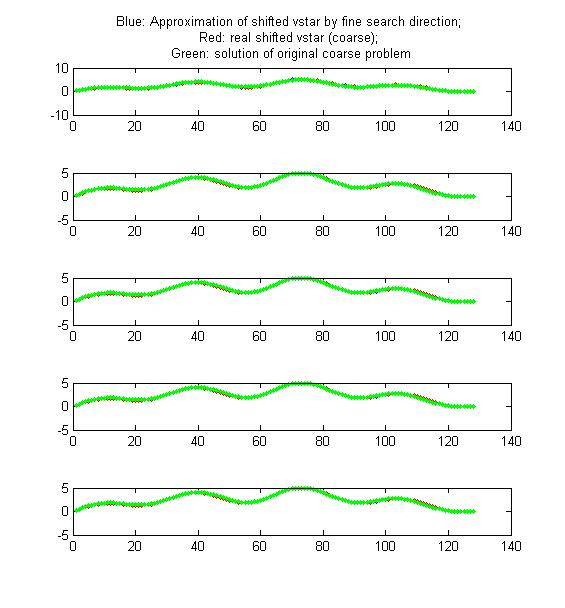
\includegraphics[width=0.6\textwidth]{coarsevscom257fig}}
  \subfloat[search direction]
  {\label{fig:direction}
  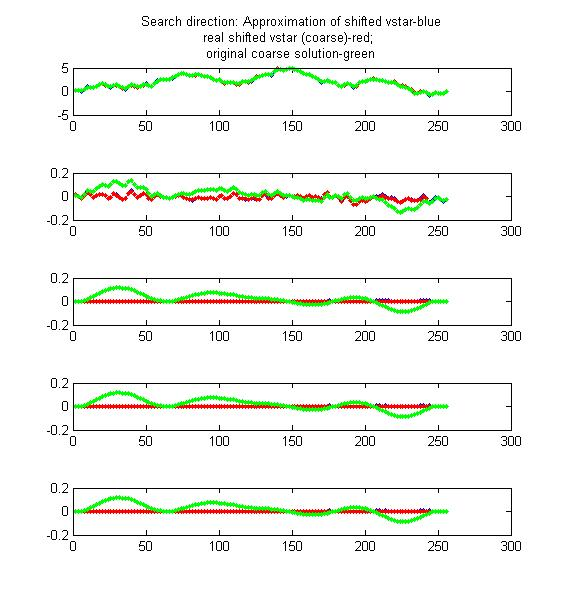
\includegraphics[width=0.6\textwidth]{coarsedirection257com}}
  \caption{2-side bounds: TN: lin1; MG/OPT: lin3; Compare solution in coarse grid: discretization level: $[257,128]$}
  \label{fig:coarse}
\end{figure}



\bf{Output of 5th cycle of MG/OPT:}
\begin{quote}
\begin{verbatim}
In  mgrid: n = 257
  it     nf     cg           f           |g|
   0      1      0   -5.66763126e+004   1.4e+003
   1      2      2   -5.66763126e+004   1.4e+003
 
#################################
### NO EXTRA BOUND CONSTRAINT ###
#################################
 
In  mgrid: n = 128
  it     nf     cg           f           |g|
   0      1      0   -2.82421049e+004   4.1e+002
   1      2      4   -2.82423697e+004   4.1e+002
   2      3     54   -2.82424262e+004   2.8e+002
   3      4     57   -2.82424520e+004   1.3e+002
   4      5     59   -2.82425721e+004   7.7e+001
   5      6     61   -2.82426652e+004   6.3e+000
   6      7     63   -2.82426666e+004   1.5e+000
   7      8     67   -2.82426668e+004   5.5e-001
   8      9     76   -2.82426668e+004   4.3e-001
   9     10     87   -2.82426669e+004   5.1e-001
  10     11    130   -2.82426669e+004   5.5e-001
  11     12    180   -2.82426669e+004   4.7e-001
  12     13    228   -2.82426669e+004   4.0e-001
  13     14    250   -2.82426669e+004   4.2e-001
  14     15    270   -2.82426669e+004   4.3e-001
  15     16    305   -2.82426669e+004   2.0e-001
  16     17    338   -2.82426669e+004   2.5e-001
  17     18    341   -2.82426669e+004   2.5e-001
  18     19    364   -2.82426669e+004   6.5e-002
  19     20    367   -2.82426669e+004   6.1e-002
  20     21    380   -2.82426669e+004   5.3e-002
  21     22    384   -2.82426669e+004   5.5e-002
  22     23    397   -2.82426669e+004   8.2e-002
  23     24    409   -2.82426669e+004   4.1e-002
  24     25    419   -2.82426669e+004   5.0e-002
  25     26    432   -2.82426669e+004   4.1e-002
  26     27    445   -2.82426669e+004   3.7e-002
  27     28    448   -2.82426669e+004   2.9e-002
  28     29    460   -2.82426669e+004   2.5e-002
  29     30    474   -2.82426669e+004   1.2e-002
  30     31    491   -2.82426669e+004   8.1e-003
  31     32    505   -2.82426669e+004   2.2e-003
  32     33    524   -2.82426669e+004   1.8e-003
  33     34    535   -2.82426669e+004   1.2e-003
  34     35    564   -2.82426669e+004   6.4e-004
  35     36    589   -2.82426669e+004   5.6e-004
  36     37    592   -2.82426669e+004   4.0e-004
MG/Opt line search: alpha =  1.00000000e+000
In  mgrid: n = 257
  it     nf     cg           f           |g|
   0      1      0   -5.66769813e+004   1.4e+003
   1      2      2   -5.66769813e+004   1.4e+003

-------------------
Optimization costs per grid
-------------------
N:        257   128
-------------------
NF(it):    10   196
NF(nf):    20   215
NF(cg):    20  3241
-------------------
\end{verbatim}
\end{quote}


\section{TN: lin3; MG/OPT:lin3}

\bf{Output of 1st cycle of MG/OPT working on $[257,128]$:}

\begin{quote}
\begin{verbatim}
In  mgrid: n = 257
  it     nf     cg           f           |g|
   0      1      0    4.62493224e+006   2.9e+005
   1      2      2    1.73085726e+005   2.3e+004
 
#################################
### NO EXTRA BOUND CONSTRAINT ###
#################################
 
In  mgrid: n = 128
  it     nf     cg           f           |g|
   0      1      0    6.40004590e+004   1.4e+004
   1      2      2   -1.71052746e+003   2.6e+003
   2      3     10   -1.81946179e+004   3.5e+003
   3      4     21   -1.83931932e+004   3.6e+003
   4      5     32   -1.93133518e+004   3.5e+003
   5      7     34   -1.93683526e+004   3.5e+003
   6      8     41   -1.99913485e+004   4.0e+003
   7      9     48   -2.07860842e+004   3.3e+003
   8     10     55   -2.14226947e+004   3.4e+003
   9     11     61   -2.18994247e+004   3.2e+003
  10     12     65   -2.19230171e+004   3.8e+003
  11     13     75   -2.25369984e+004   3.2e+003
  12     14     81   -2.27217905e+004   3.2e+003
  13     15     86   -2.29434215e+004   3.2e+003
  14     16     90   -2.30641974e+004   3.0e+003
  15     17     94   -2.31568892e+004   3.0e+003
  16     18     98   -2.32879819e+004   3.0e+003
alpha0 =
     1
Error in Line Search (lmqnbcm.m)
    ncg1   = 4
    alpha  =   0.00000000
    alpha0 =   1.00000000
    g'p    = -2.9169e+003
    |g|     =  1.0321e+004
    |p|     =  5.9334e-001
MG/Opt line search: alpha =  1.00000000e+000
In  mgrid: n = 257
  it     nf     cg           f           |g|
   0      1      0   -1.35218465e+004   2.2e+004
   1      2      2   -4.28115105e+004   3.6e+003

-------------------
Optimization costs per grid
-------------------
N:        257   128
-------------------
NF(it):     2    16
NF(nf):     4    18
NF(cg):     4   102
-------------------
\end{verbatim}
\end{quote}

\bf{Output of 5th cycle of MG/OPT:}
\begin{quote}
\begin{verbatim}
In  mgrid: n = 257
  it     nf     cg           f           |g|
   0      1      0   -5.68043929e+004   7.0e+001
   1      2      4   -5.68045459e+004   2.8e+001
 
#################################
### NO EXTRA BOUND CONSTRAINT ###
#################################
 
In  mgrid: n = 128
  it     nf     cg           f           |g|
   0      1      0   -2.82490033e+004   3.9e+002
   1     10     50   -2.82490566e+004   4.6e+002
alpha0 =
     1
Error in Line Search (lmqnbcm.m)
    ncg1   = 2
    alpha  =   0.00000000
    alpha0 =   1.00000000
    g'p    = -2.4109e+002
    |g|     =  4.8517e+002
    |p|     =  3.5303e+000
MG/Opt line search: alpha =  1.25000000e-001
In  mgrid: n = 257
  it     nf     cg           f           |g|
   0      1      0   -5.68045463e+004   2.8e+001
   1      2      7   -5.68046214e+004   1.3e+001

-------------------
Optimization costs per grid
-------------------
N:        257   128
-------------------
NF(it):    10    80
NF(nf):    20   108
NF(cg):    56   541
-------------------

\end{verbatim}
\end{quote}


\begin{figure}
  \centering
  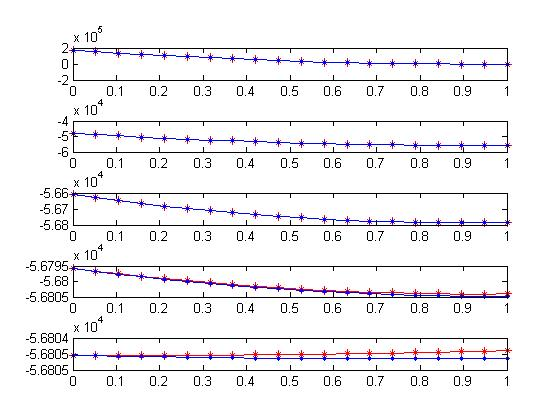
\includegraphics[width=1\textwidth]{merit33}
  \caption{2-side bounds: TN: lin3; MG/OPT: lin3; penalty $\rho=1$, merit and objective function based on different $\alpha$}
  \label{fig:merit33}
\end{figure}

\begin{figure}[H]
  \centering
  \subfloat[solution]
  {\label{fig:vsc}
  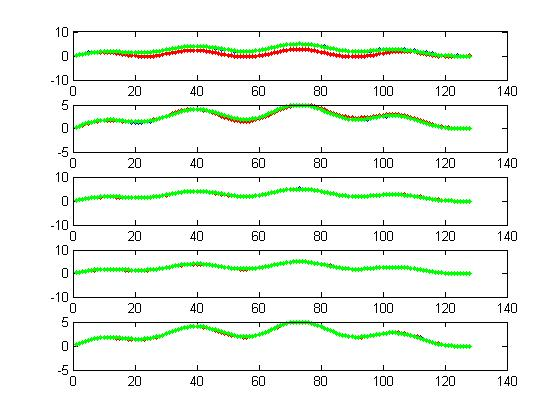
\includegraphics[width=0.6\textwidth]{coarsevs33}}
  \subfloat[search direction]
  {\label{fig:direction}
  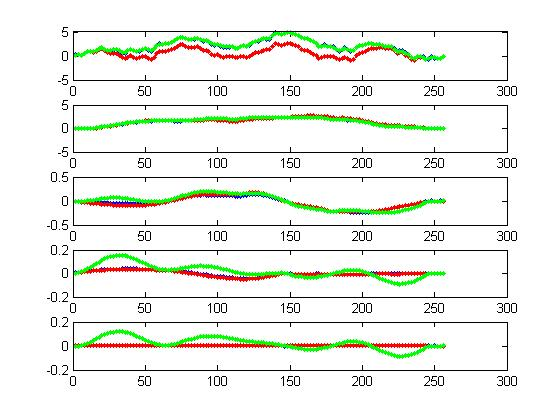
\includegraphics[width=0.6\textwidth]{coarsedir33}}
  \caption{2-side bounds: TN: lin3; MG/OPT: lin3; Compare solution in coarse grid: discretization level: $[257,128]$}
  \label{fig:coarse33}
\end{figure}

\begin{figure}
  \centering
  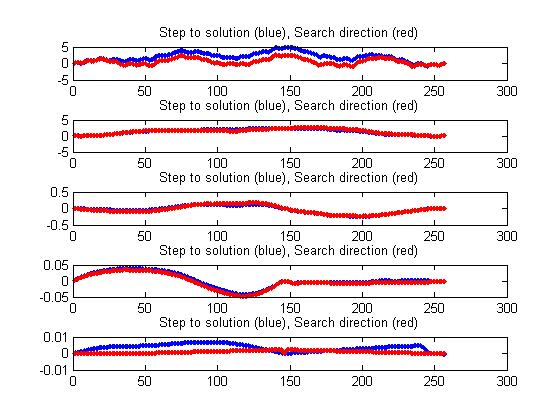
\includegraphics[width=1\textwidth]{finedirvs25733}
  \caption{2-side bounds: TN: lin3; MG/OPT: lin3; Compare step to solution with search direction on fine level: discretization level: $[257,128]$}
  \label{fig:fine}
\end{figure}

\section{TN: lin2; MG/OPT: lin3}
\bf{Output of 5th cycle:}
\begin{quote}
\begin{verbatim}
In  mgrid: n = 257
  it     nf     cg           f           |g|
   0      1      0   -5.68046940e+004   8.6e+000
   1      2     21   -5.68047254e+004   4.4e+000
 
#################################
### NO EXTRA BOUND CONSTRAINT ###
#################################
 
In  mgrid: n = 128
  it     nf     cg           f           |g|
   0      1      0   -2.82491963e+004   4.0e+002
   1      2     50   -2.83680035e+004   2.0e+002
   2      3     75   -2.83862763e+004   6.5e+001
   3      4    101   -2.83912259e+004   5.1e+001
   4      5    117   -2.83916011e+004   4.6e+001
   5      6    134   -2.83916553e+004   4.3e+001
   6      7    170   -2.83917090e+004   6.0e+000
   7      8    211   -2.83917212e+004   3.6e+000
   8      9    240   -2.83917252e+004   3.7e+000
   9     10    262   -2.83917278e+004   6.1e+000
  10     11    282   -2.83917308e+004   4.1e+000
  11     12    312   -2.83917363e+004   2.0e+000
  12     13    325   -2.83917371e+004   1.6e+000
  13     14    347   -2.83917378e+004   1.1e+000
  14     15    361   -2.83917382e+004   1.0e+000
  15     16    374   -2.83917386e+004   6.7e-001
  16     17    394   -2.83917390e+004   1.2e+000
  17     18    409   -2.83917393e+004   4.6e-001
  18     19    426   -2.83917395e+004   4.1e-001
  19     20    440   -2.83917395e+004   2.6e-001
  20     21    474   -2.83917398e+004   3.7e-001
  21     22    498   -2.83917399e+004   2.5e-001
  22     23    519   -2.83917400e+004   1.4e-001
  23     24    569   -2.83917401e+004   2.2e-001
  24     25    604   -2.83917401e+004   1.0e-001
  25     26    630   -2.83917401e+004   6.3e-002
  26     27    650   -2.83917401e+004   4.7e-002
  27     28    668   -2.83917401e+004   2.7e-002
  28     29    680   -2.83917401e+004   7.1e-003
  29     30    704   -2.83917401e+004   9.6e-003
  30     31    724   -2.83917401e+004   3.6e-003
  31     32    740   -2.83917401e+004   1.8e-003
  32     33    751   -2.83917401e+004   1.1e-003
  33     34    770   -2.83917401e+004   1.3e-003
  34     35    785   -2.83917401e+004   4.4e-004
In  mgrid: n = 257
  it     nf     cg           f           |g|
   0      1      0   -5.68047254e+004   4.4e+000
   1      2     20   -5.68047317e+004   1.4e+000

-------------------
Optimization costs per grid
-------------------
N:        257   128
-------------------
NF(it):    10   185
NF(nf):    20   196
NF(cg):    73  3781
-------------------
\end{verbatim}
\end{quote}

As the above output shown, we can see that coarse level approximation couldn't provide a descent direction to fine level even though $e'*Gvmg<0$. 

\begin{figure}[H]
  \centering
  \subfloat[solution]
  {\label{fig:vsc}
  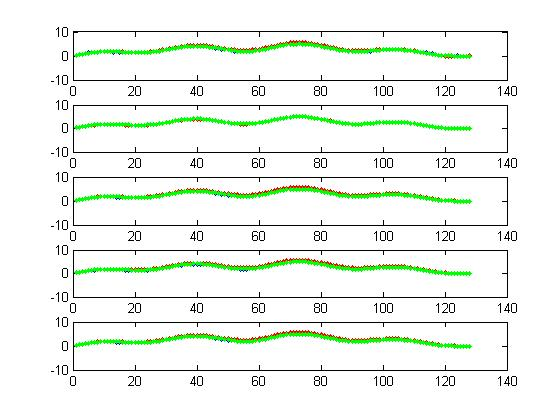
\includegraphics[width=0.6\textwidth]{coarsevs23}}
  \subfloat[search direction]
  {\label{fig:direction}
  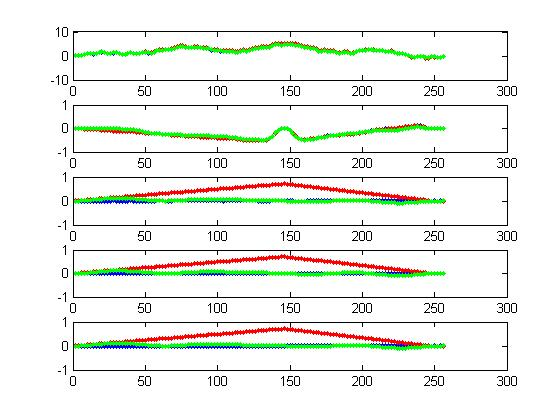
\includegraphics[width=0.6\textwidth]{coarsedir23}}
  \caption{2-side bounds: TN: lin2; MG/OPT: lin3; Compare solution in coarse grid: discretization level: $[257,128]$}
  \label{fig:coarse23}
\end{figure}

\begin{figure}
  \centering
  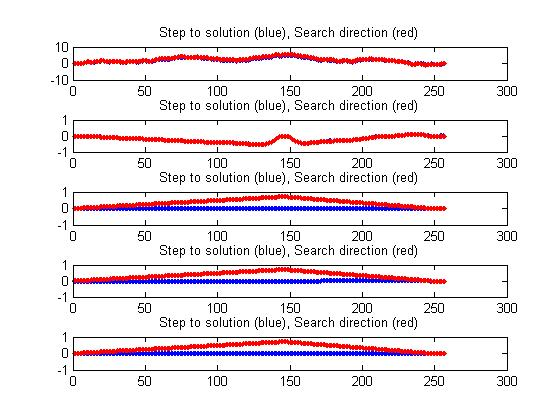
\includegraphics[width=1\textwidth]{finedirvs23}
  \caption{2-side bounds: TN: lin2; MG/OPT: lin3; Compare step to solution with search direction on fine level: discretization level: $[257,128]$}
  \label{fig:fine23}
\end{figure}

 
\begin{figure}
  \centering
  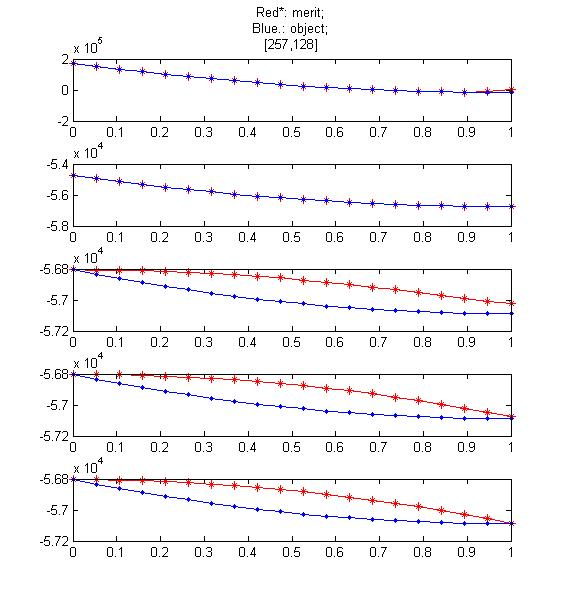
\includegraphics[width=1\textwidth]{merit23}
  \caption{2-side bounds: TN: lin2; MG/OPT: lin3; penalty $\rho=1$, merit and objective function based on different $\alpha$}
  \label{fig:merit23}
\end{figure}


\section{1-side bound: TN: lin1; MG/OPT: lin2}

\begin{figure}[H]
  \centering
  \subfloat[solution]
  {\label{fig:vsc1s12}
  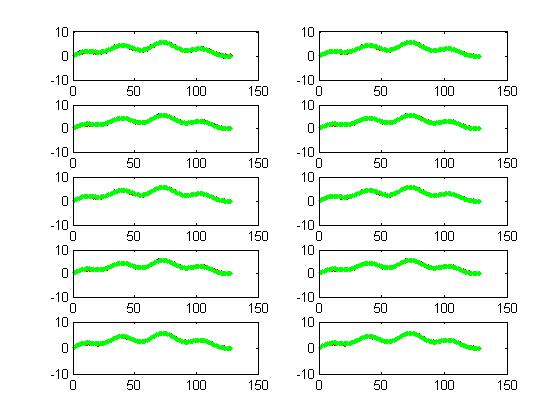
\includegraphics[width=0.6\textwidth]{coarsevs1s12}}
  \subfloat[search direction]
  {\label{fig:direction1s12}
  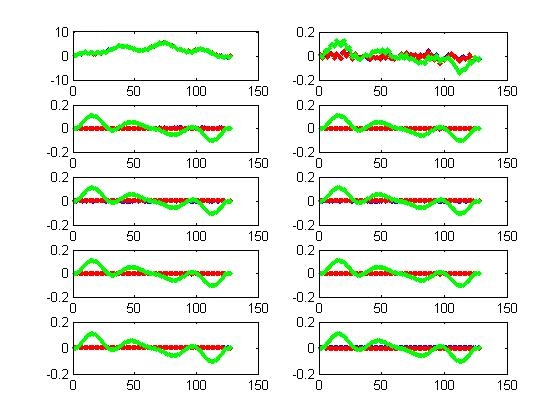
\includegraphics[width=0.6\textwidth]{coarsedir1s12}}
  \caption{1-side bound constraint: TN: lin1; MG/OPT: lin2; Compare solution in coarse grid: discretization level: $[257,128]$}
  \label{fig:coarse1s12}
\end{figure}

\begin{figure}
  \centering
  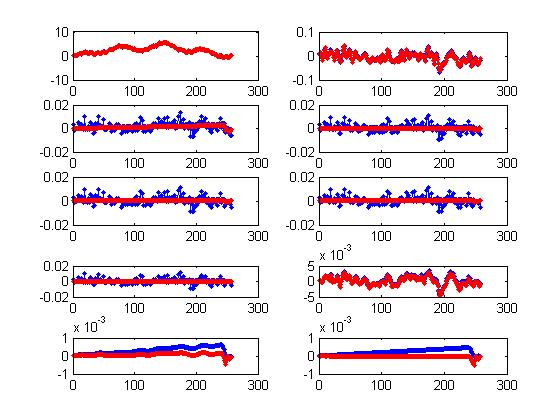
\includegraphics[width=1\textwidth]{finedir1s12}
  \caption{1-side bound constraint: TN: lin1; MG/OPT: lin2;  Compare step to solution with search direction on fine level: discretization level: $[257,128]$}
  \label{fig:fine1s12}
\end{figure}

 
\begin{figure}
  \centering
  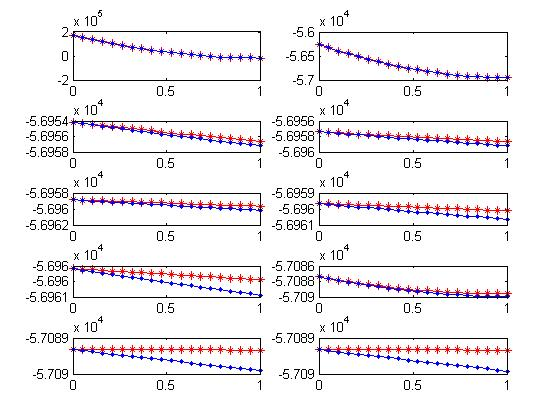
\includegraphics[width=1\textwidth]{merit1s12}
  \caption{1-side bound constraint: TN: lin1; MG/OPT: lin2;  penalty $\rho=1$, merit and objective function based on different $\alpha$}
  \label{fig:merit12}
\end{figure}

\section{1-side bound: TN: lin2; MG/OPT: lin2}

\begin{figure}[H]
  \centering
  \subfloat[solution]
  {\label{fig:vsc1s22}
  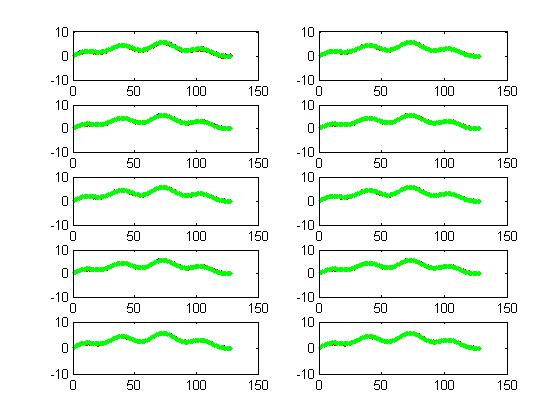
\includegraphics[width=0.6\textwidth]{coarsevs1s22}}
  \subfloat[search direction]
  {\label{fig:direction1s22}
  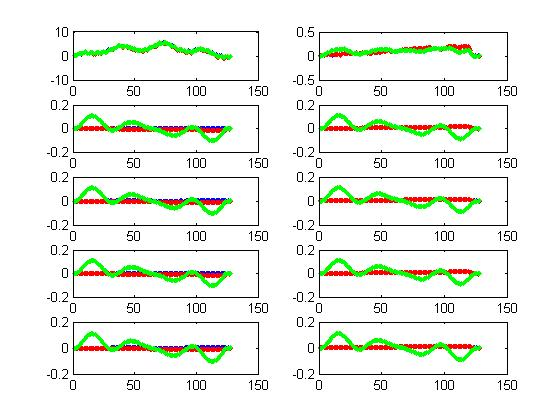
\includegraphics[width=0.6\textwidth]{coarsedir1s22}}
  \caption{1-side bound constraint:  TN: lin2; MG/OPT: lin2; Compare solution in coarse grid: discretization level: $[257,128]$}
  \label{fig:coarse1s22}
\end{figure}

\begin{figure}
  \centering
  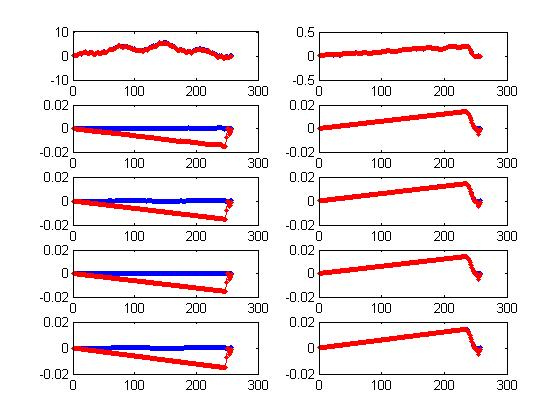
\includegraphics[width=1\textwidth]{finedir1s22}
  \caption{1-side bound constraint:   TN: lin2; MG/OPT: lin2; Compare step to solution with search direction on fine level: discretization level: $[257,128]$}
  \label{fig:fine1s22}
\end{figure}

 
\begin{figure}
  \centering
  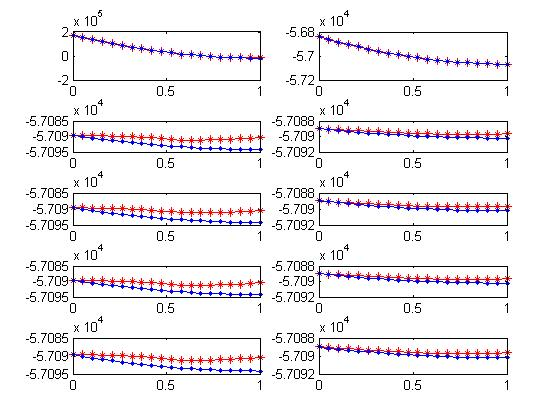
\includegraphics[width=1\textwidth]{merit1s22}
  \caption{1-side bound constraint:   TN: lin2; MG/OPT: lin2; penalty $\rho=1$, merit and objective function based on different $\alpha$}
  \label{fig:merit22}
\end{figure}

\section{1-side bound: TN: lin3; MG/OPT: lin2}

\begin{figure}[H]
  \centering
  \subfloat[solution]
  {\label{fig:vsc1s32}
  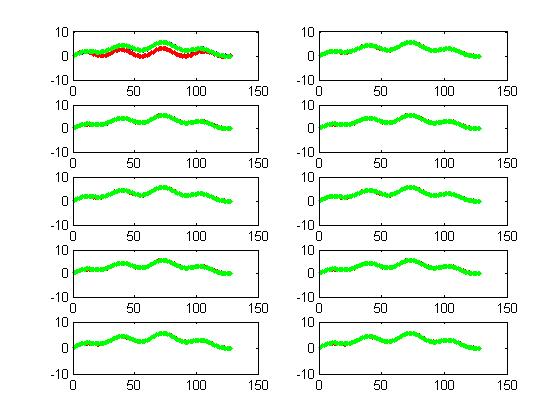
\includegraphics[width=0.6\textwidth]{coarsevs1s32}}
  \subfloat[search direction]
  {\label{fig:direction1s32}
  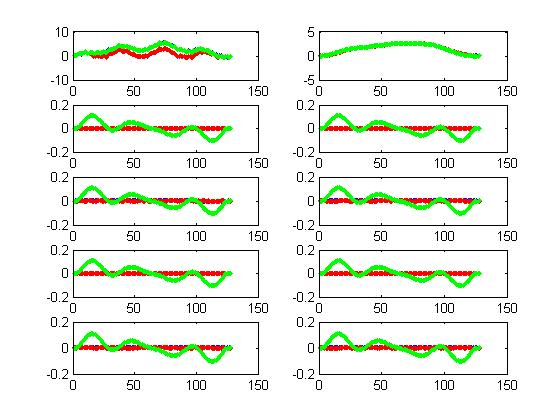
\includegraphics[width=0.6\textwidth]{coarsedir1s32}}
  \caption{1-side bound constraint:   TN: lin3; MG/OPT: lin2; Compare solution in coarse grid: discretization level: $[257,128]$}
  \label{fig:coarse1s32}
\end{figure}

\begin{figure}
  \centering
  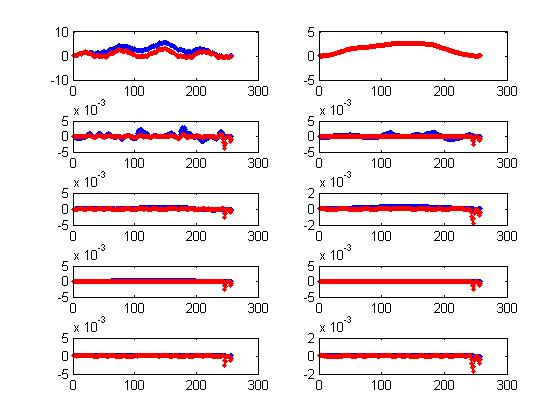
\includegraphics[width=1\textwidth]{finedir1s32}
  \caption{1-side bound constraint:  TN: lin3; MG/OPT: lin2; Compare step to solution with search direction on fine level: discretization level: $[257,128]$}
  \label{fig:fine1s32}
\end{figure}

 
\begin{figure}
  \centering
  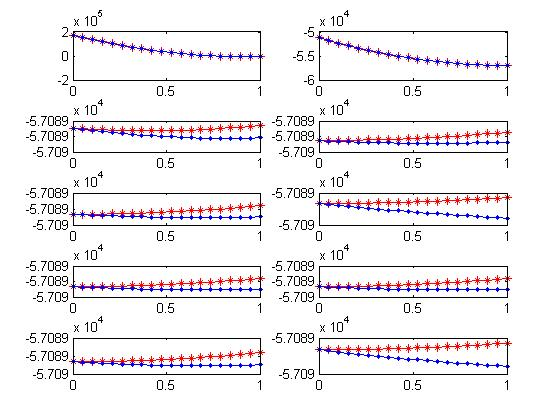
\includegraphics[width=1\textwidth]{merit1s32}
  \caption{1-side bound constraint: TN: lin3; MG/OPT: lin2;  penalty $\rho=1$, merit and objective function based on different $\alpha$}
  \label{fig:merit32}
\end{figure}



\bf{Output of 10th cycle: TN: lin3; MG/OPT: lin2}
\begin{quote}
\begin{verbatim}
In  mgrid: n = 257
  it     nf     cg           f           |g|
   0      1      0   -5.70896641e+004   1.4e-002
   1      2     50   -5.70896641e+004   2.7e-002
 
#################################
### NO EXTRA BOUND CONSTRAINT ###
#################################
 
In  mgrid: n = 128
  it     nf     cg           f           |g|
   0      1      0   -2.83884805e+004   2.6e+002
   1      4      3   -2.83885960e+004   2.7e+002
alpha0 =
     1
Error in Line Search (lmqnbcm.m)
    ncg1   = 2
    alpha  =   0.00000000
    alpha0 =   1.00000000
    g'p    = -3.4021e+000
    |g|     =  3.0168e+002
    |p|     =  1.3446e-002
only lower violation
only lower violation
only lower violation
only lower violation
only lower violation
only lower violation
only lower violation
only lower violation
only lower violation
only lower violation
only lower violation
only lower violation
only lower violation
only lower violation
only lower violation
only lower violation
only lower violation
only lower violation
only lower violation
only lower violation
only lower violation
only lower violation
only lower violation
only lower violation
only lower violation
only lower violation
only lower violation
only lower violation
only lower violation
only lower violation
only lower violation
only lower violation
MG/Opt line search: alpha =  2.44140625e-004
In  mgrid: n = 257
  it     nf     cg           f           |g|
   0      1      0   -5.70896641e+004   2.7e-002
   1      2     30   -5.70896641e+004   1.1e-002

-------------------
Optimization costs per grid
-------------------
N:        257   128
-------------------
NF(it):    20    92
NF(nf):    40   113
NF(cg):   417   998
-------------------
\end{verbatim}
\end{quote}










\end{document}

